%\documentclass[<options>]{elsarticle}
\documentclass [sort&compress] {elsarticle}
\usepackage{graphicx}% Include figure files

\bibliographystyle{elsarticle-num}
\begin{document}
\begin{frontmatter}

%\title{Influence of $\gamma$--irradiation and ultrasound treatment on carrier transport in Au�-SiO$_2$�-Si structure}

\title{Influence of $\gamma$--irradiation and ultrasound treatment on current mechanism in  Au�-SiO$_2$�-Si structure}


\author{A.M.~Gorb}
\author{O.A.~Korotchenkov}

\author{O.Ya.~Olikh\corref{cor1}}
\ead{olikh@univ.kiev.ua}

\author{A.O.~Podolian}
\author{R.G.~Chupryna}



\cortext[cor1]{Corresponding author}



\address{Faculty of Physics, Taras Shevchenko National University of Kyiv, Kyiv 01601, Ukraine}


\begin{abstract}
The effect of  $^{60}$Co $\gamma$--irradiation ($5\cdot10^7$~rad) and ultrasound treatment (4~MHz, 2~W/cm$^2$, up to 60 min) on current--voltage characteristics is experimentally investigated in an Au�-SiO$_2$�-Si structure.
The change in the current mechanism is analysed in terms of a modifying defect system.
The irradiation is shown to enhance the space charge limited current and trap--assisted tunneling current.
Experimental observations of the acoustically induced low temperature annealing of 
the $P_b$ and $E'$ centers, which causes the partial recovery of irradiated silicon MOS structure characteristics, are highlighted.
\end{abstract}




\begin{keyword}
MOS structures\sep Si�-SiO$_2$ interface\sep ultrasound treatment\sep $\gamma-$rays
\end{keyword}


\end{frontmatter}


\section{Introduction}

It is well known that defects are crucial for semiconductor devices performance. 
Thus, electrical characteristics of metal--oxide--semiconductor (MOS) structure are  extremely sensitive to the interface state density. 
The formation of radiation defects (RDs) near the interface is therefore very harmful for device fabrications and frequently leads to a change in current mechanisms \cite{Rao,Tascioglu2010old,Tataroglu:2007NIMA,Olikh:2013IEEE,Verma,Abdolahpour}.
It is known that elastic acoustic vibrations can effectively interact with RDs and offer an interesting approach in trying to develop novel tools to controllably manipulate the defect properties. 
For example, RDs were annealed by acoustic wave treatments at a much lower temperature compared to that used for thermal annealing. 
Such phenomenon was observed in Si \cite{Podolian2012, PodolHivrEn, YOlikh2006TPL}, Ge \cite{Olikh:FTP1996}, semiconducting compounds \cite{OlikhProc, OstrovFTTRad}, and alkali halides \cite{UST:OstrovCsI}. 
Usually, the suggested mechanism deals with a decay of radiation--formed complexes and acoustically induced (AI) diffusion of defects to a sink.

Moreover, the ultrasound treatment (UST) can recover defect-related electronic parameters of irradiated barrier structures.
For example, the "active" ultrasound effects were observed in solar cells \cite{Davletova2009,Davletova2008,YOlikh2007TPL,Olikh2018JAP}, 
light-emitting diodes (LEDs) \cite{US:LED,UST:LED_SM}, 
and Schottky diodes \cite{Pashaev2014,Olikh:Ultras}. 
Furthermore, the AI modification of interface defects \cite{Ostap:SiO2,UST:Medvid,Zaver:2008} and minority carrier lifetimes \cite{Parchinskii2003,Zdeb1989,Gorb2010} were reported in industrially important Si--SiO$_2$ system.

Particular attention was paid to the UST of silicon MOS structures irradiated by $^{60}$Co $\gamma$--rays \cite{Parchinskii2000,Parchinskii2006}.
Utilising capacitance�-voltage measurements, the authors observed the post--UST decrease of the radiation--induced charge in dielectric layers of the structures. 
They also detected decreased carrier lifetimes in Si, whereas the growth of surface recombination rates considered insignificant \cite{Parchinskii2000,Parchinskii2006}.

The first aim of our work is to experimentally investigate the influence of UST on the charge transfer in irradiated Au--SiO$_2$--Si structures.
In contrast to the cited study \cite{Parchinskii2000,Parchinskii2006}, 
our results are obtained
i)~for structures with a significantly higher RD concentration in the conductive layer (see Section~\ref{Exp});
ii)~for the diode operating in the current mode.
It should be noted that some of our results have been reported earlier \cite{Gorb2010}. 
However, this paper is focused on evolving more detailed models that describe the modification of current mechanisms and the evolution of the defect structure, which are caused by irradiation and UST.

On the other hand, the efficiency of Si solar cell is restricted
by the recombination of carriers \cite{COLLETT201750}.
The silicon surface is often highly recombination active due to the abundance of  dangling bonds.
The number of band--gap states can be reduced by introducing a dielectric coating.
The anneal is one of the most effective methods of passivation of Si--SiO$_2$ interface \cite{COLLETT201750,Kerr_2001,Aberle2000}.
This reaction was reported to release atomic hydrogen that is then free to diffuse across the oxide and passivate dangling bonds at the oxide--silicon interface \cite{Kerr_2001,Aberle2000,Larionova2010}.
The results presented in this work demonstrate the feasibility of the acoustically induced enhancement of hydrogen diffusion. 
Therefore, acousto--anneal can be used as an effective processing step in fabricating devices based on the MOS technology.



\section{Experimental and calculation details}
\label{Exp}

Experiments were performed on $n$-type (111)--oriented crystalline float-zone Si with residual boron (B) impurity concentration of about $10^{12}$~cm$^{-3}$ and doping phosphorus (P)
impurity concentration of $2\cdot10^{12}$~cm$^{-3}$.
The corresponding resistivity is $4000$~$\Omega\cdot$cm.
A bulk silicon material was divided into several rectangular--shaped samples of approximately
$1\times5\times10$~mm$^3$.
The MOS structures were formed by chemical etching of the upper Si surfaces using
HF-HNO$_3$--CH$_3$COOH solutions (HF:HNO$_3$:CH$_3$COOH~$=3:5:3$), followed by the surface oxidation due to the exposure to ambient air for 24 hours at room temperature and the Au vacuum evaporation.
As a result, SiO$_2$ layer with a thickness of $10-15$~{\AA} \cite{angermann2016,Philipossian,Morita1990} was formed.
According Sze and Lee \cite{Sze2012},
the thickness of the depletion layer is about 10~$\mu$m.
GaZn--eutectic Ohmic contacts were rubbed on the bottom surfaces of the samples.

The samples were $\gamma$--irradiated ($^{60}$Co source) at nominal room temperature to the dose of $5\cdot10^7$~rad.
The measurement on the reference bulk sample shown that the conductivity has been reduced to about 0.5 of the initial value after irradiation.
As mentioned above, the ultrasound influence on $\gamma$--irradiated Si--SiO$_2$ structure, created by thermal oxidation, has been previously investigated \cite{Parchinskii2000,Parchinskii2006}.
However, we used higher irradiation dozes, up to $5\cdot10^7$~rad, which were not more than $10^6$~rad in Refs. \cite{Parchinskii2000,Parchinskii2006}.
Second, the sample resistivity was much greater in our case ($4000$~$\Omega\cdot$cm in contrast to $0.2-0.5$~$\Omega\cdot$cm reported in Refs. \cite{Parchinskii2000,Parchinskii2006}); 
therefore, the non--ionizing energy losses were larger as well.
Third, it is known \cite{PersenkovBook} that the density of $\gamma$--induced interface defects depends on substrate orientation, and an irradiation of (111)--oriented Si--SiO$_2$ structure (our case) leads to higher RD concentrations compared to that for the (100) substrate employed by Parchinskii \textit{et al}. \cite{Parchinskii2000,Parchinskii2006}. 
Therefore, much more heavy structure degradation is expected in our case.

UST was done by attaching the piezoelectric transducer to one side of the sample.
An epoxy glue was used as the bonding medium, providing the rigid coupling of the transducer to the sample.
The thickness resonance of the transducers was 4~MHz.
A radio--frequency voltage supplied from a generator drives the transducer, resulting in vibrations of the coupled transducer-sample system.
UST was carried out by a two consecutive loading--unloading cycles, 30~min each;
so the total UST time $t_\mathrm{UST}$ was equal to either 30~min or 60~min.
The acoustic energy flux density $W_{US}$ in Si was about 2~W/cm$^2$.
The sample temperature was measured with a copper--constantan thermocouple directly attached to the surface and did not exceed 350~K.
The more details about the sample and UST setup are given elsewhere \cite{Gorb2010}.

The initial Au�-SiO$_2$�-Si structure, $\gamma$--irradiated structure, and both irradiated and ultrasonically treated structure were investigated by using the  current--voltage ($I$--$V$) technique.
The forward and reverse bias characteristics were measured at 300~K in the current range from $10^{-9}$ to $10^{-3}$~A with a voltage step of $0.01$~V.
To identify the current mechanism in the irradiated structure, $I$--$V$ characteristics were measured over a temperature range $\sim$300-340~K before UST.


The data non--linear fitting was done by using the method of modified artificial bee colony \cite{MABC}.


\section{Results and Discussion}


Fig.~\ref{figIV} shows the $I$--$V$ characteristics taken in the initial and irradiated Au--SiO$_2$--Si structures as well as after the sequent USTs.
It is seen that the $I$--$V$ curve for the non--irradiated sample is typical for the Schottky diode:
The forward current is caused by a thermionic emission (TE) over the potential barrier,
the reverse current value is determined by the barrier height lowering, which occurs due to the electric field ($\log I\sim V^{1/2}$) \cite{Rhoderick1988,Andrews}.
The forward branch was modeled by fitting the following equation to the experimental data plotted in Fig.~\ref{figIV} \cite{Rhoderick1988}
\begin{equation}
\label{eqSDIV}
I=I_s\left\{\exp\left[\frac{q(V-IR_s)}{nkT}\right]-1\right\}\,,
\end{equation}
where
$I_s$ is the saturation current,
$R_s$ is the series resistance,
$n$ is the ideality factor,
the other symbols  have their usual meanings.
The fitting results are shown by solid lines in Fig.~\ref{figIV}(b) and (d),
the resulting parameter values are listed in Table~\ref{tabMIS}.
It should be noted that the presence of the oxide layer does not allow the barrier height to be determined only using the $I_s$ value,
since the carrier tunneling must also be taken into account \cite{OZBEK2011,Kobayashi}.



\begin{figure}
\centerline{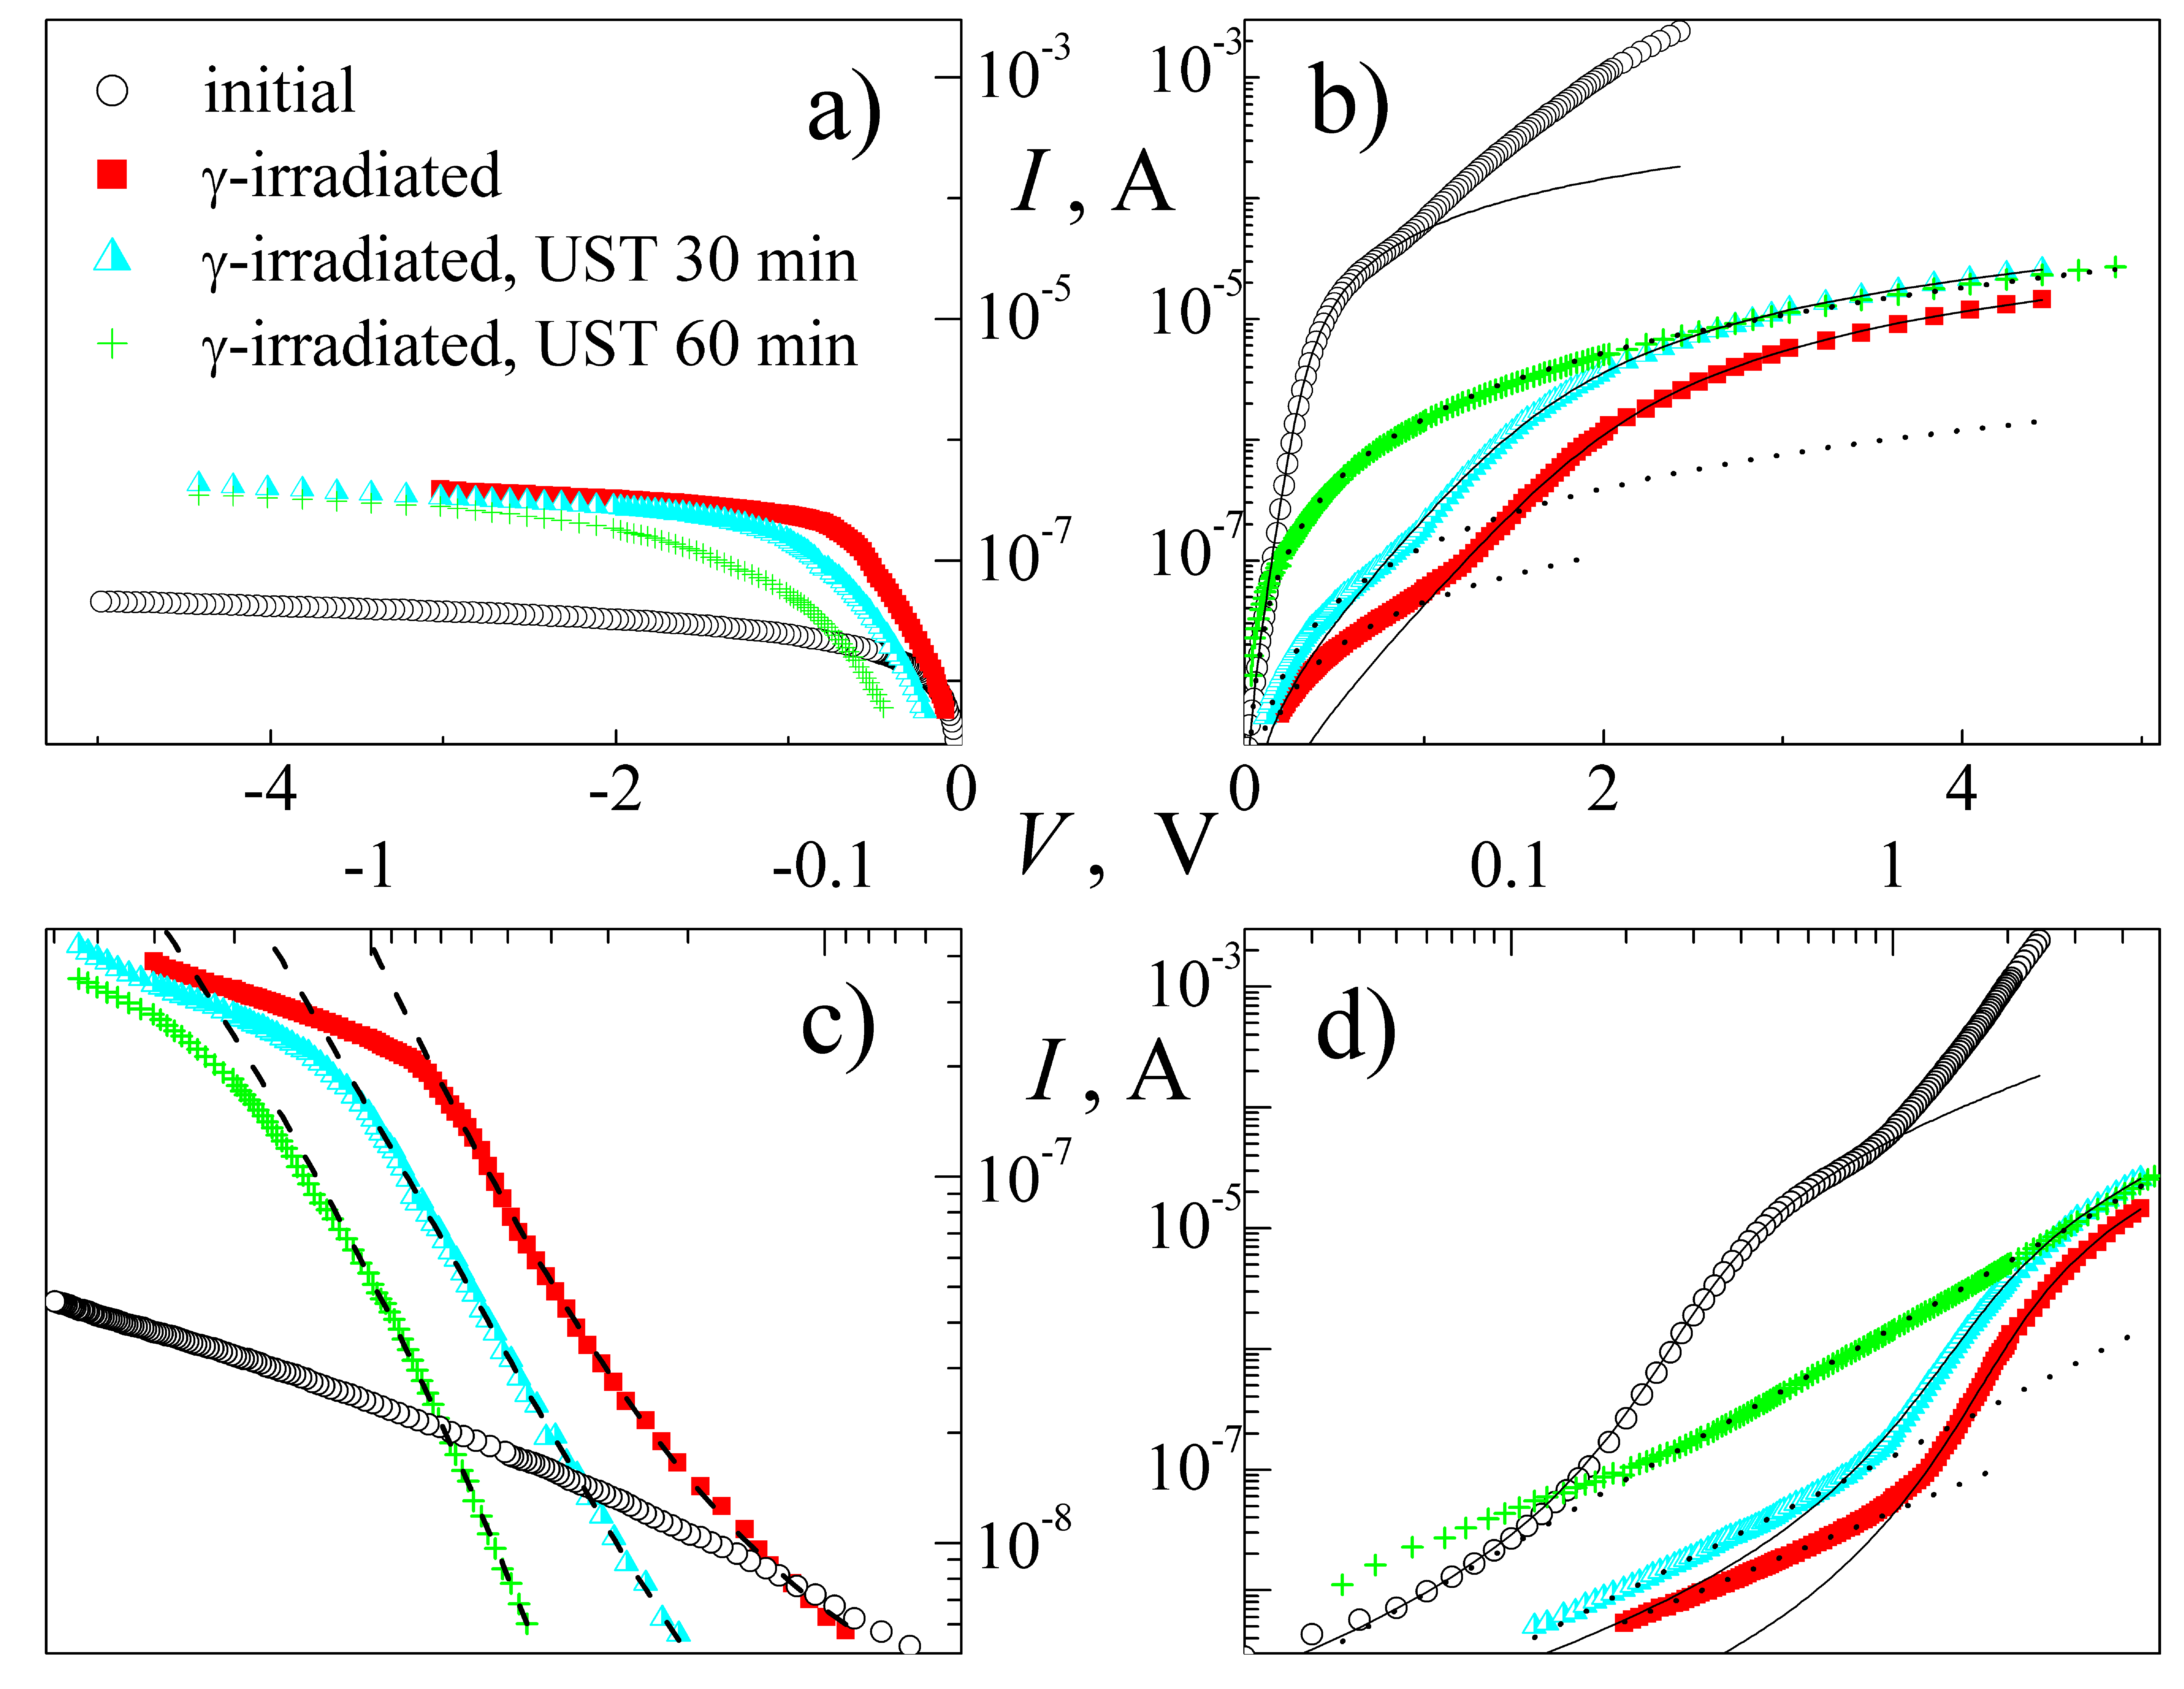
\includegraphics[width=0.95\textwidth]{figIV}}
\caption{\label{figIV}
The logarithmical (a, b) and double-logarithmical (c, d) plots of the reverse (a, c) and forward (b, d) $I$--$V$ characteristics for Au--SiO$_2$--Si structure before and after $\gamma$--irradiation and UST.
$T=300$~K.
The marks are the experimental results,
and the solid, dashed, and dotted lines are the TE, TAT, and SCLC fitted curves using Eqs.~(\ref{eqSDIV}), (\ref{eqIVTAT}), and (\ref{eqVIsclc}), respectively.
}%
\end{figure}



\begin{table}
\caption{\label{tabMIS}Extracted parameters for the Au--SiO$_2$--Si structure
}
\center
\begin{tabular}{lcccc}
\hline
\multicolumn{5}{l}{Structure status}\\\hline
$\gamma$--irradiation&$-$&$+$&$+$&$+$\\
UST&$-$&$-$&$+$&$+$\\
$t_\mathrm{UST}$ (min)&$0$&$0$&30&60\\ \hline
\multicolumn{5}{l}{Parameter}\\\hline
$I_s$ ($10^{-9}$A) & $3.3\pm0.3$& $1.1\pm0.2$& $4.9\pm0.5$&$-$ \\
$R_s$ ($10^{4}$��) & $1.1\pm0.2$& $13\pm1$& $9\pm1$&$-$ \\
$n$ & $1.7\pm0.1$& $10.3\pm0.2$& $9.9\pm0.2$& \\
$m_\mathrm{F}$ &$-$ &$1.30\pm0.05$& $1.6\pm0.05$& $1.8\pm0.05$ \\
$I_0$ ($10^{-8}$A) &$-$ &$5\pm1$& $13\pm2$& $150\pm10$ \\
$I_{0,\mathrm{TAT}}$ (a.u.) &$-$ &1& $0.14\pm0.03$& $0.04\pm0.01$ \\
$U_d$ (V) &$-$ &$0.7\pm0.1$& $0.44\pm0.05$& $0.12\pm0.05$ \\
$R_\mathrm{TAT}$ (a.u.) & &1& $0.54\pm0.05$& $0.33\pm0.04$ \\
$K_{\mathrm{RECT},\,\,0.5\mathrm{V}}$ &$800\pm100$ &$0.22\pm0.03$& $1.3\pm0.2$& $5.4\pm0.8$ \\
\end{tabular}
\end{table}


The experimental forward current value obtained in the non--irradiated structure exceeds the one expected from Eq.~(\ref{eqSDIV}) at high bias; see Fig.~\ref{figIV}.
The extra current is most likely to be due to the carrier tunneling through the SiO$_2$ layer.
The tunneling current can be given by \cite{Rhoderick1988,Novikov2009}:
\begin{equation}\label{eqFowlNord}
    \ln\left(\frac{I}{F_m^2}\right)\propto -\frac{4 \sqrt{2m^*}(qE_{\mathrm{eff}})^{3/2}}{3\hbar q F_m}\,,
\end{equation}
where
$F_m$ is the electric field,
$E_{\mathrm{eff}}$ is the effective tunneling energy.
The linearity of the Fowler--Nordheim plot (Fig.~\ref{FigFauler})  indicates  of reasonable assumption for the excess current mechanism.
It was taken into account when plotting that the electric field in a oxide layer is proportional to the applied voltage $F_m\propto V$.


\begin{figure}
\centerline{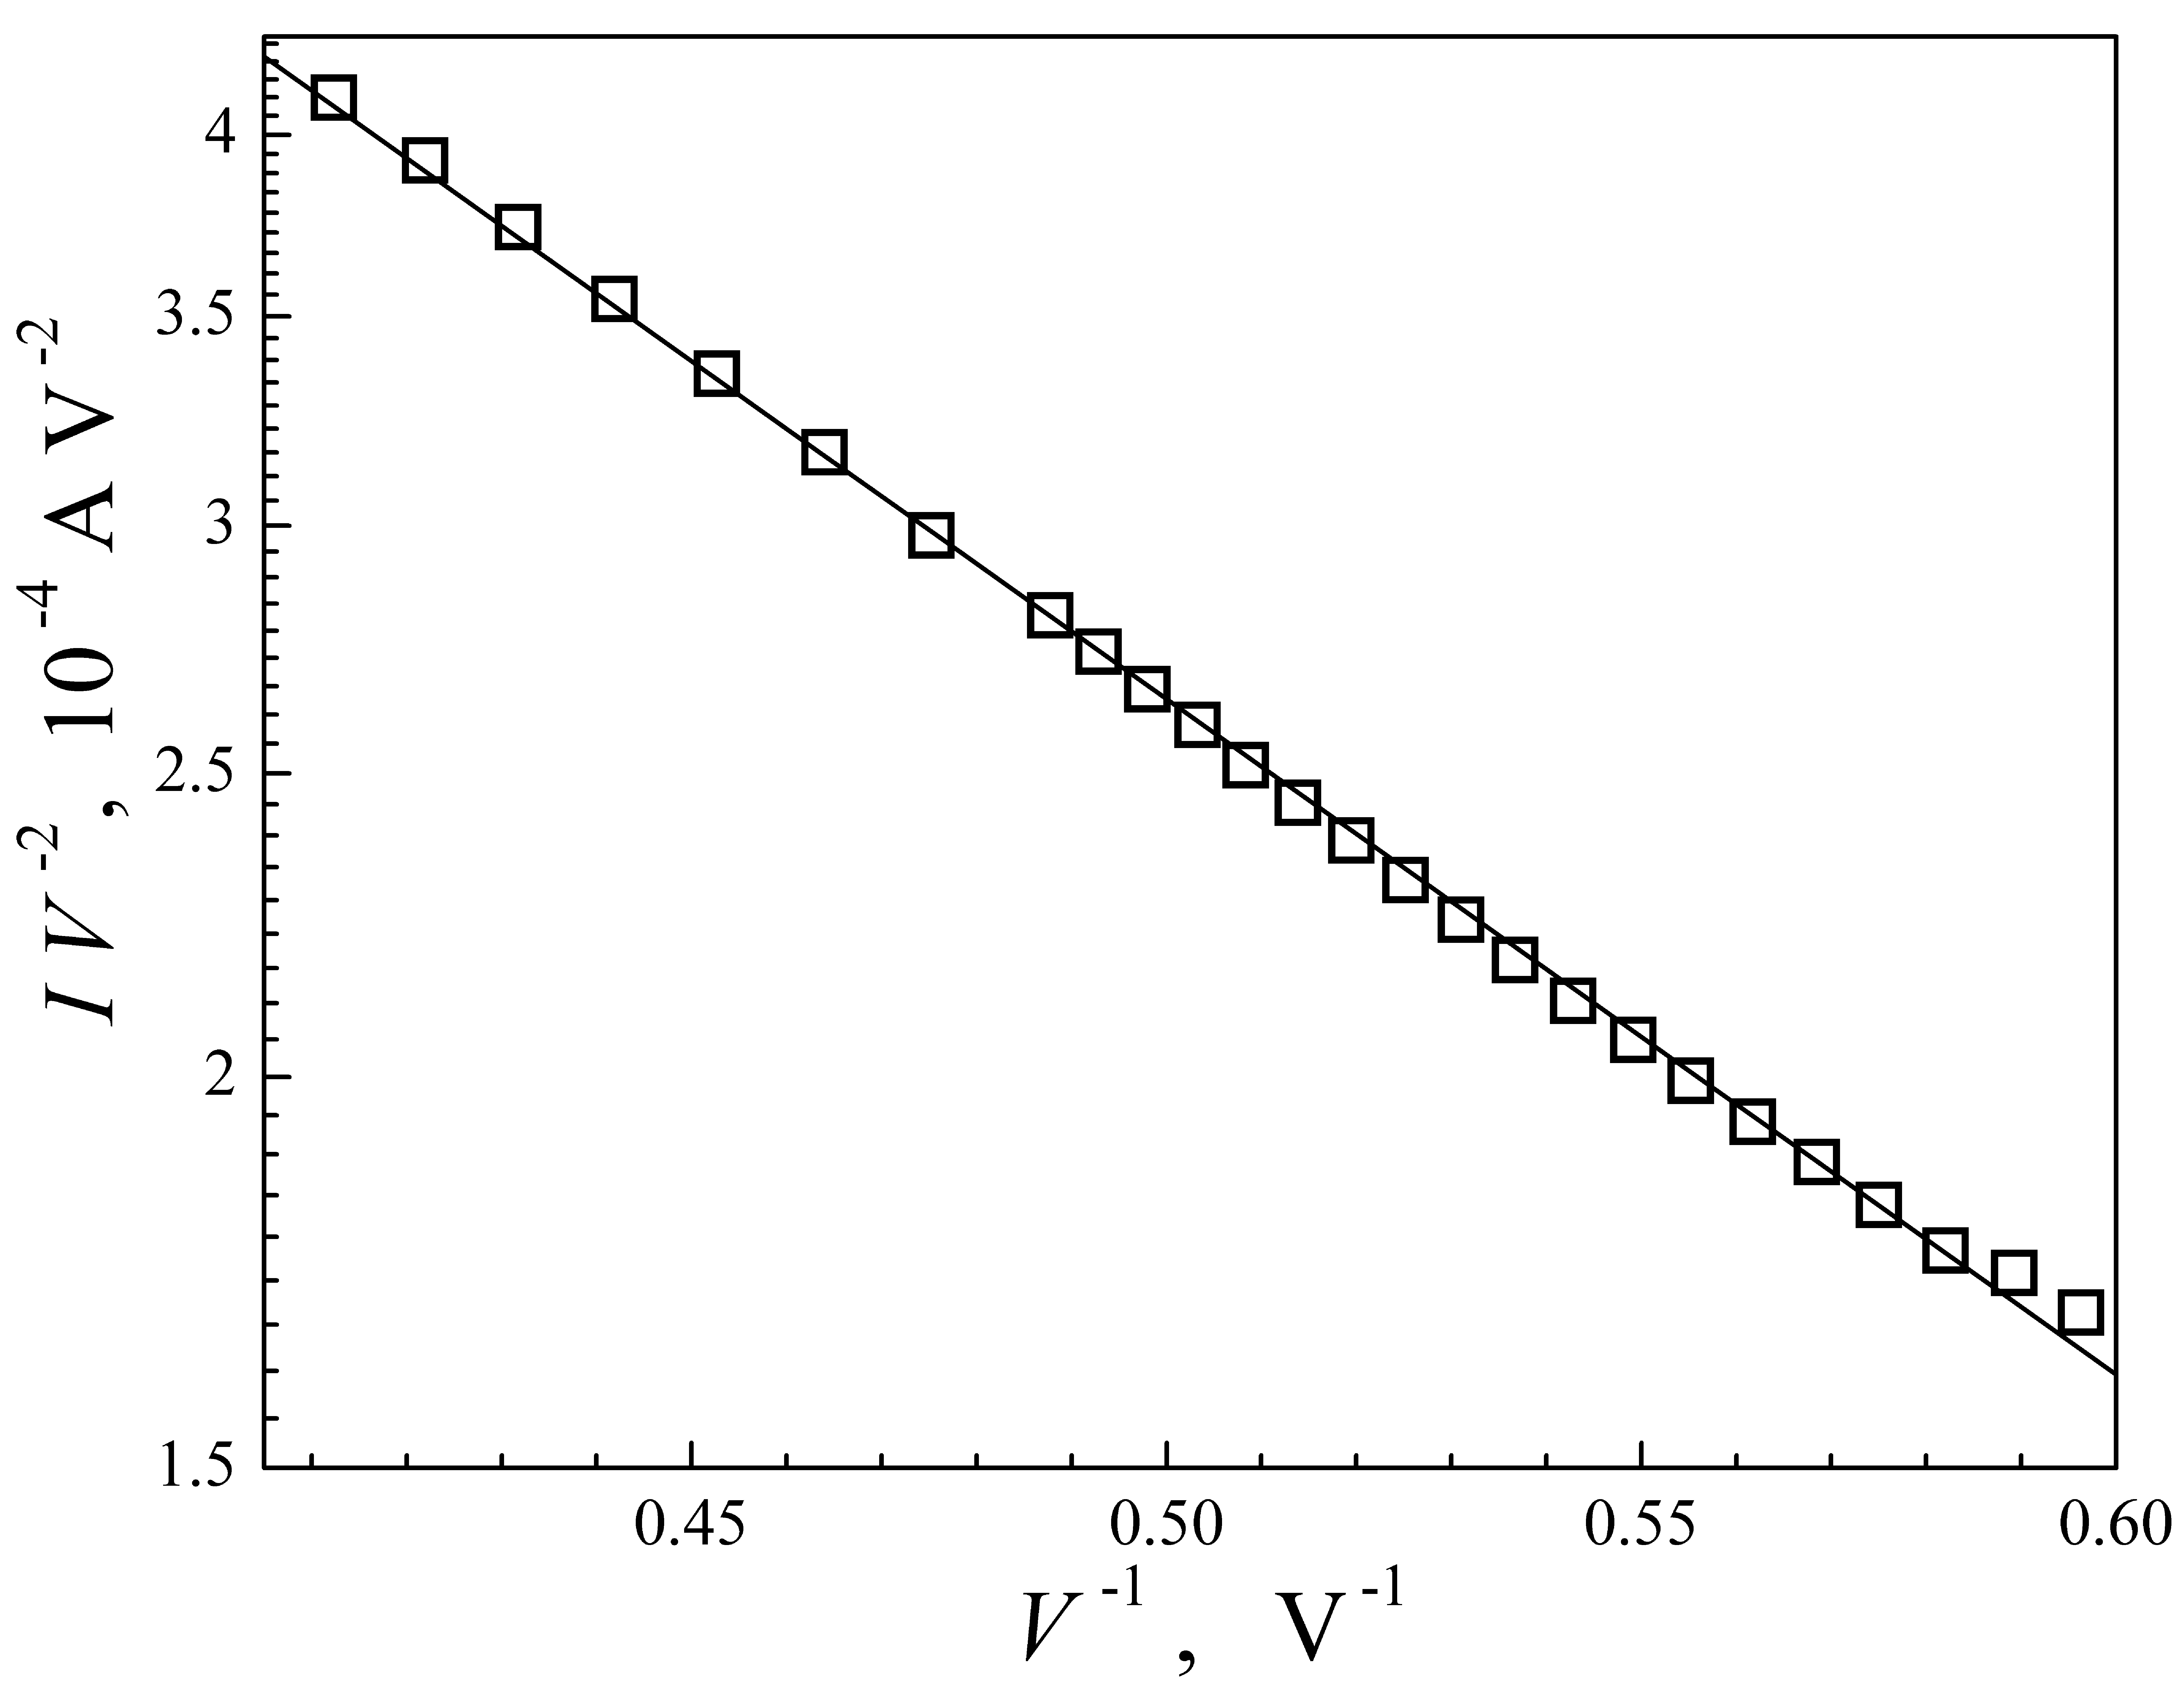
\includegraphics[width=0.6\textwidth]{FigFauler}}
\caption{\label{FigFauler}
The Fowler-Nordheim plot of the forward branch for the non--irrradiated Au--SiO$_2$--Si structure at $V>1,6$~V.
The line is the least--squares linear fitting result.
}%
\end{figure}

As shown in Fig.~\ref{figIV}, the $\gamma$--irradiation has a considerable effect on the
$I$--$V$ curve, which is obviously due to a modified current mechanism.
Thus, the forward current decreases after irradiation and the $I$--$V$ dependence, which is expected in the TE model, is observed only at $V>1$~V.
It should be emphasised that the radiation--induced current reduction in MOS structure was previously reported \cite{SiO2:Niu}.


The region $V>1$~V fitted by Eq.~(\ref{eqSDIV}) shows that the irradiation can significantly increase both the series resistance and ideality factor; see Table~\ref{tabMIS}.
In our opinion, increase in $R_s$ can be explained by the $\gamma$--irradiation effects in bulk Si.
Pintilie \emph{et al}. \cite{FZSi:Rad} investigated the influence of $\gamma$--irradiation ($9\cdot10^7$~rad) on silicon (Fz--Si, $4$~k$\Omega\cdot$cm),
demonstrating that the known complexes VO$_i$, C$_i$C$_s$, $H$--center (V$_2$O$_i$), $\Gamma$--center, and interstitial defect $I^{0/-}$ are the main radiation defects involved.
$I^{0/-}$ is a secondary defect and its appearance leads to compensation (inversion) of electrical conductivity \cite{FZSi:Rad}.
It may be suggested that this defect is responsible for varying series resistance $R_s$.
In turn, the increase in $R_s$ to about 13 times causes the reduction of the voltage drop in the dielectric layer.
As a result, the electric field intensity was ceased to be sufficient for effective Fowler--Nordheim tunneling and such current component was not observed after irradiation.
The increase in the ideality factor can also be explained by formation of RDs and results in observed decreasing of the TE current.

Fig.~\ref{figIV}(d) shows that the forward $I$--$V$ characteristic of irradiated structures at low biases ($V<1$~V) is quite well described by a power law
\begin{equation}\label{eqVIsclc}
  I=I_0\,V^{\,m_\mathrm{F}},
\end{equation}
where
$m_\mathrm{F}=\frac{V}{I}\frac{\partial V}{\partial I}$ is the power--law parameter.
The relation (\ref{eqVIsclc}) is typical for the space charge limited current
(SCLC) \cite{SCLC:MA2016,Jafar,SCLC:Kaya} with the value of $m_\mathrm{F}$ being the energy distribution of traps emitting carriers.
For instance, the value $m_\mathrm{F}\approx1.3$, which is observed in our structure after $\gamma$--irradiation and before UST corresponds to the exponentially distributed traps.
It is known \cite{SCLC:MA2016,Jafar,SCLC:Kaya} that $I_0$ depends on the total trap concentration $N_t$ as
\begin{equation}\label{eqIoSCLC}
  I_0\sim 1/N_t^{m_\mathrm{F}-1},
\end{equation}
and the temperature dependence of the power--law parameter is given by
\begin{equation}\label{eqMT_IoSCLC}
  m_\mathrm{F}=1+T_c/T,
\end{equation}
where
$T_c$ is the trap energy distribution parameter.
This can be related to the trap concentration per unit energy range located at an energy $E$ above the valence band maximum as $P(E)=\frac{N_t}{kT_c}\exp(-\frac{E}{kT_c})$.
The observed linearity of the temperature dependence of $m_\mathrm{F}$ (inset in Fig.~\ref{figEa_MIS}) supports the above assumption that the SCLC would be taken into account to explain the experiments.
It is also known \cite{Jafar} that the SCLC conduction should become important when the
density of injected carriers is much larger than the density of thermally generated carriers.
Therefore, SCLC appearance be expected in our structures fabricated on Si substrates with a high resistivity.

The SCLC current--voltage relation is often written as \cite{Jafar}
\begin{equation}\label{eqVIsclcT}
  I(V,T)=C\exp\left(-\frac{E_x}{kT}\right)\,V^{\,m_\mathrm{F}(T)},
\end{equation}
where
$C$ is the constant and
$E_x$ is the activation energy linked to the trap level.
Taking into account Eq.~(\ref{eqMT_IoSCLC}), one gets the temperature dependence of the forward current shown in Fig.~\ref{figEa_MIS}.
It is seen that the experimental data points in Fig.~\ref{figEa_MIS} can be fitted well by Eq.~(\ref{eqVIsclcT}) (line in Fig.~\ref{figEa_MIS}) with the fitting parameter $E_x=(0,32\pm0,01)$~eV.



\begin{figure}
\centerline{
\includegraphics[width=0.6\textwidth]{figEa_MIS}}
\caption{\label{figEa_MIS}
Temperature dependence of SCLC--current for $\gamma$--irrradiated Au--SiO$_2$--Si structure before UST at $V=0,4$~V.
Inset: Temperature dependence of power--law parameter.
Lines are the least--squares linear fits.
}%
\end{figure}

Let's consider radiation defects, which can result in SCLC.
Some notes are appropriate.
Firstly, the low temperature and low partial oxygen pressure used here form thin SiO$_2$ layers.
Meanwhile, same radiation defects are known \cite{SiO2:Cantin} to be  created in both thin and thick layers.
Secondly, the hydrogen content is the key factor for generating electrically active RDs in Si---MOS structures \cite{SiO2:Cantin}.
Native SiO$_2$ layers are known to be enriched with atomic hydrogen \cite{angermann2016,PersenkovBook}.


The $\gamma$--irradiation of Si--SiO$_2$ structures is known \cite{PersenkovBook} to lead to
a stress relaxation, trap filling, and charged defect generation.
It is believed \cite{SiO2:Devine,SiO2:Lenahan} that the negative charge is trapped at the interface while the positive charge accumulates in the oxide bulk.
In particular, the irradiation results in breaking of the $\equiv\!\mathrm{Si}\!-\!\mathrm{H}$ bonds at Si--SiO$_2$ interface \cite{SiO2:Mahapatra,SiO2:Esseni,Fleetwood}.
The unsaturated bonds $\equiv\mathrm{Si}-$ act as electronic traps.
The configuration of these defects depends appreciably on the silicon substrate orientation.
It is widely believed \cite{SiO2:Rev} that the $P_b$ centers appear at the (111)--oriented substrate interface, 
whereas the $P_{b1}$ and $P_ {b0}$ centers are typical for the (100)--oriented substrates.
Both $P_ {b0}$ and $P_{b1}$ are chemically identical to $P_b$,
although the difference in their electrical activity has been observed \cite{SiO2:Rev}.
The anneal temperature is about 150$^\circ$C \cite{Fleetwood} for $P_b$.

The $\gamma$--ray irradiation with doses above $5\cdot10^5$~rad leads to non--monotonic energy distribution of interface levels in  $n$--Si---SiO$_2$ structure \cite{PersenkovBook}.
According to Parchinskii \emph{et al}. \cite{ParchSiO2}, the highest density of surface states is observed at $E_c-(0,32\pm0,04)$~eV, coinciding with the value of $E_x$ obtained from Fig.~\ref{figEa_MIS}.


In our opinion, the $P_b$ traps, being main electronic traps, are involved in SCLC process at low forward bias in irradiated structures.
Besides, the negative charge accumulated at the interface results both in increasing the barrier height and decreasing the TE current.


Figs.~\ref{figIV}(b) and (d) show that 
UST causes an increase in the space charge limited current.
We used Eq.~(\ref{eqVIsclc}) to fit experimental $I$--$V$ curves of ultrasonically treated structures.
The resulting fitting parameters are summarized in Table~\ref{tabMIS}.
According to Eq.~(\ref{eqIoSCLC}), the detected increase in the $I_0$ value is evidently due to AI decreased $P_b$ concentration.
It should be pointed out that acousto--annealing takes place at rather low temperatures, which do not exceed $\approx$80$^\circ$C.

On the one hand, 
the acousto-�defect interaction in Si has been reported \cite{Roman:2010JAP,Korotchenkov1995,Olikh2009Sem,UST:Medvid,OlikhJAP,Savkina2015}
to cause atomic diffusion, transformation of native and impurity defects,
modification of interior surface states, and appearance of new defects.
On the other hand,
the $P_b$ center annealing is known \cite{SiO2:Takakura,SiO2:Wurzer} to deal with the passivation of dangling bonds at the oxide--silicon interface by hydrogen atoms.
Therefore, the AI diffusion of hydrogen can be attempted to explain our results. 
It should be stressed that similar phenomenon has previously been reported \cite{Ostap:SiO2,Ostap:PhotoLum,ostapenko1997}.

Table~\ref{tabMIS} shows that UST leads to the increase of $m_\mathrm{F}$.
According to Eq.~(\ref{eqMT_IoSCLC}), the $m_\mathrm{F}$ increment deals with the increase in $T_c$ value as well as narrowing of the distribution of trap levels.
So, it is known \cite{Jafar} that $m_\mathrm{F}=2$ is observed in the case of single--energy traps.
Therefore, the acousto--annealing selectivity is evidenced by the observed narrowing,
so that atomic hydrogen can be captured only by certain dangling bonds during UST.

In our opinion, the key parameter for the AI bond passivation is an existence of mechanical stress, which is generally non--uniform at the interface.
The impurity diffusivity in turn depends on the stress \cite{AZIZ2001}.
The varying mechanical stress at acoustic loading can displace the hydrogen atoms, and the efficiency of AI passivation is therefore determined by the strain field around the defect.

The acousto--annealing of the $P_b$ centers decreases the negative interface charge 
and results both in partial recovery of the barrier height and increase in the TE current value; see Table~~\ref{tabMIS}. 
The AI decrease in $R_s$ is therefore due to annealing of RDs ($I^{0/-}$ center) in the bulk of silicon.


The $\gamma$--released hydrogen atoms are potentially hazardous because of these mobile species are able \cite{SiO2:Devine,SiO2:DiMaria,SiO2:Mahapatra,SiO2:Esseni}
i)~to interact with hydrogen bonded at the Si/SiO$_2$ interface and thus to give rise to additional $P_b$ centers;
ii)~to move inside the semiconductor bulk and to produce generation--recombination  sites  and deactivate boron in  the Si  substrate;
iii)~to migrate within oxide thus creating the $E'$ centers.
It is believed \cite{SiO2:Takakura,SiO2:Devine} that the $E'$ center is due to broken $\equiv\!\mathrm{Si}\!-\!\mathrm{O}$ bonds,
resulting from the oxygen vacancy in SiO$_2$ and trapping positive charge.
It has been concluded \cite{Fleetwood,SiO2:Devine} that the $E'$ centers dominate the hole trapping processes in oxide films grown on silicon.
In $10^{7}$~rad $\gamma$--irradiated silicon, the total concentration of $E'$ is about $10^{18}$~cm$^{-3}$, but the centers are non--uniformly distributed over the oxide layer depth and
largest concentrations are expected near the Si/SiO$_2$  interface  \cite{PersenkovBook}.
The broken $\equiv\!\mathrm{Si}\!-\!\mathrm{O}$ bonds do not recover at room temperature and the  temperature of $E'$ annealing is equal to 200$^\circ$C \cite{SiO2:Mahapatra,SiO2:Takakura,Fleetwood}.


The generation of $E'$ centers is accompanied by a large (several orders of magnitude) increase in leakage currents \cite{SiO2:Mahapatra,SiO2:DiMaria,Fleetwood}.
The leakage currents are likely caused by inelastic tunneling of conduction band electrons to defect centers in the oxide near the  Si/SiO$_2$ boundary \cite{Fleetwood,SiO2:Esseni,SiO2:DiMaria}.
In our opinion, such a trap--assisted tunneling (TAT) current is responsible for a reverse current in irradiated structures --- Figs.~\ref{figIV}(a) and \ref{figIV}(c).

In fact, according to \cite{TAT:Gilmore,TAT:GopalSST,TAT:Gopal}, the bias dependence of the TAT current is described by
\begin{equation}\label{eqIVTAT}
  I_R=I_{0,\mathrm{TAT}}\,(U_d-V)\exp\left(-\frac{R_\mathrm{TAT}}{F_m}\right),
\end{equation}
where
$I_{0,\mathrm{TAT}}$ and $R_\mathrm{TAT}$ do not depend on voltage,
$I_{0,\mathrm{TAT}}$ is proportional to the trap concentration and
$U_d$ is the barrier height.
The reverse $I$--$V$ branches for irradiated structures before and after UST were fitted to Eq.~(\ref{eqIVTAT}). 
It is seen in Fig.~\ref{figIV} that
the experimental data are in a good agreement with the fitting curves, which thus confirms the above assumption that the reverse current mechanism is involved.
The current deviation at high bias is probably caused by series resistance.

Analysing the deduced parameters listed in Table~\ref{tabMIS}, 
one can see that UST leads to decrease in the $I_{0,\mathrm{TAT}}$ and barrier height values.
The former is evidently due to low temperature acousto--annealing of radiation traps ($E'$ centers).  This can be thought to come from acoustically stimulated diffusion of interstitial oxygen and hydrogen atoms.
The barrier lowering is obviously in agreement with $P_b$ annealing mentioned above.

The analysis also show that $\gamma$--irradiation results in considerable degradation of the rectification factor $K_\mathrm{RECT}$.
But UST leads to a forward current increase as well as reverse current decrease in irradiated  Au�-SiO$_2$�-Si structures.
Weighing the $K_\mathrm{RECT}$ data at 0.5~V listed in Table~\ref{tabMIS}, we conclude that the recovery of $K_\mathrm{RECT}$ is observed due to UST.
Thereby, a partial recovery of $\gamma$--degraded Si--MOS structure properties by ultrasound treatment is observed at temperatures close to room temperature.


\section{Conclusion}
The influence of $\gamma$--irradiation and ultrasound treatment on current mechanisms in Au�-SiO$_2$�-Si structures is experimentally studied.
In the non-treated structures, the thermionic emission and tunneling through the SiO$_2$ layer contribute to the current.
It is shown that $\gamma$--irradiation results in appearance of the space charge limited current at forward bias and trap--assisted tunneling current at reverse bias as well as in attenuation of the thermionic emission current.
It is revealed that ultrasound treatments at temperatures close to room temperature increase the rectification factor value.
The observed acoustically induced variation of the current is indicative of a low--temperature ($\approx$80$^\circ$C) annealing of the $P_b$ and $E'$ centers.
These observations can be explained by an enhanced diffusivity of interstitial species (hydrogen and oxygen) under ultrasound loading conditions.
Taking into account the observed increase in the power--law parameter for a space charge limited current it can be concluded that ultrasound treatment narrows the energy distribution of $\gamma$--induced traps at the Si/SiO$_2$  interface.
Thus, ultrasound can be an effective tool for controlling metal�-semiconductor structure characteristics.

\bibliography{olikh}

\end{document}

